\section{Development \& Testing}

\subsection{Development}
Due to the pandemic we weren't able to get much experience. In 2022 we had our first real RoboCup
in the LightWeight International League. With this experience we started to design the 2023 Robot.
\newline
The design of our robots aims to be as rigid as possible, while keeping the robot light.
To achieve this goal, we used Carbon and 3D printed Parts in combination with thin circuit boards.
In combination with our Software, we are able to travel with high speeds to the ball and
hit a goal.

\subsection{Mechanical Design}
All our parts were designed using 'Autodesk Inventor 2023 Professional' and 'Autodesk Eagle 9.6.2'.
Most of our parts are printed with our Prusa MK3S+ and the Carbon rings are CNC-Machined
with our self build CNC-Machine.
\newline
\newline

\begin{wrapfigure}{r}{4cm}
    \centering
    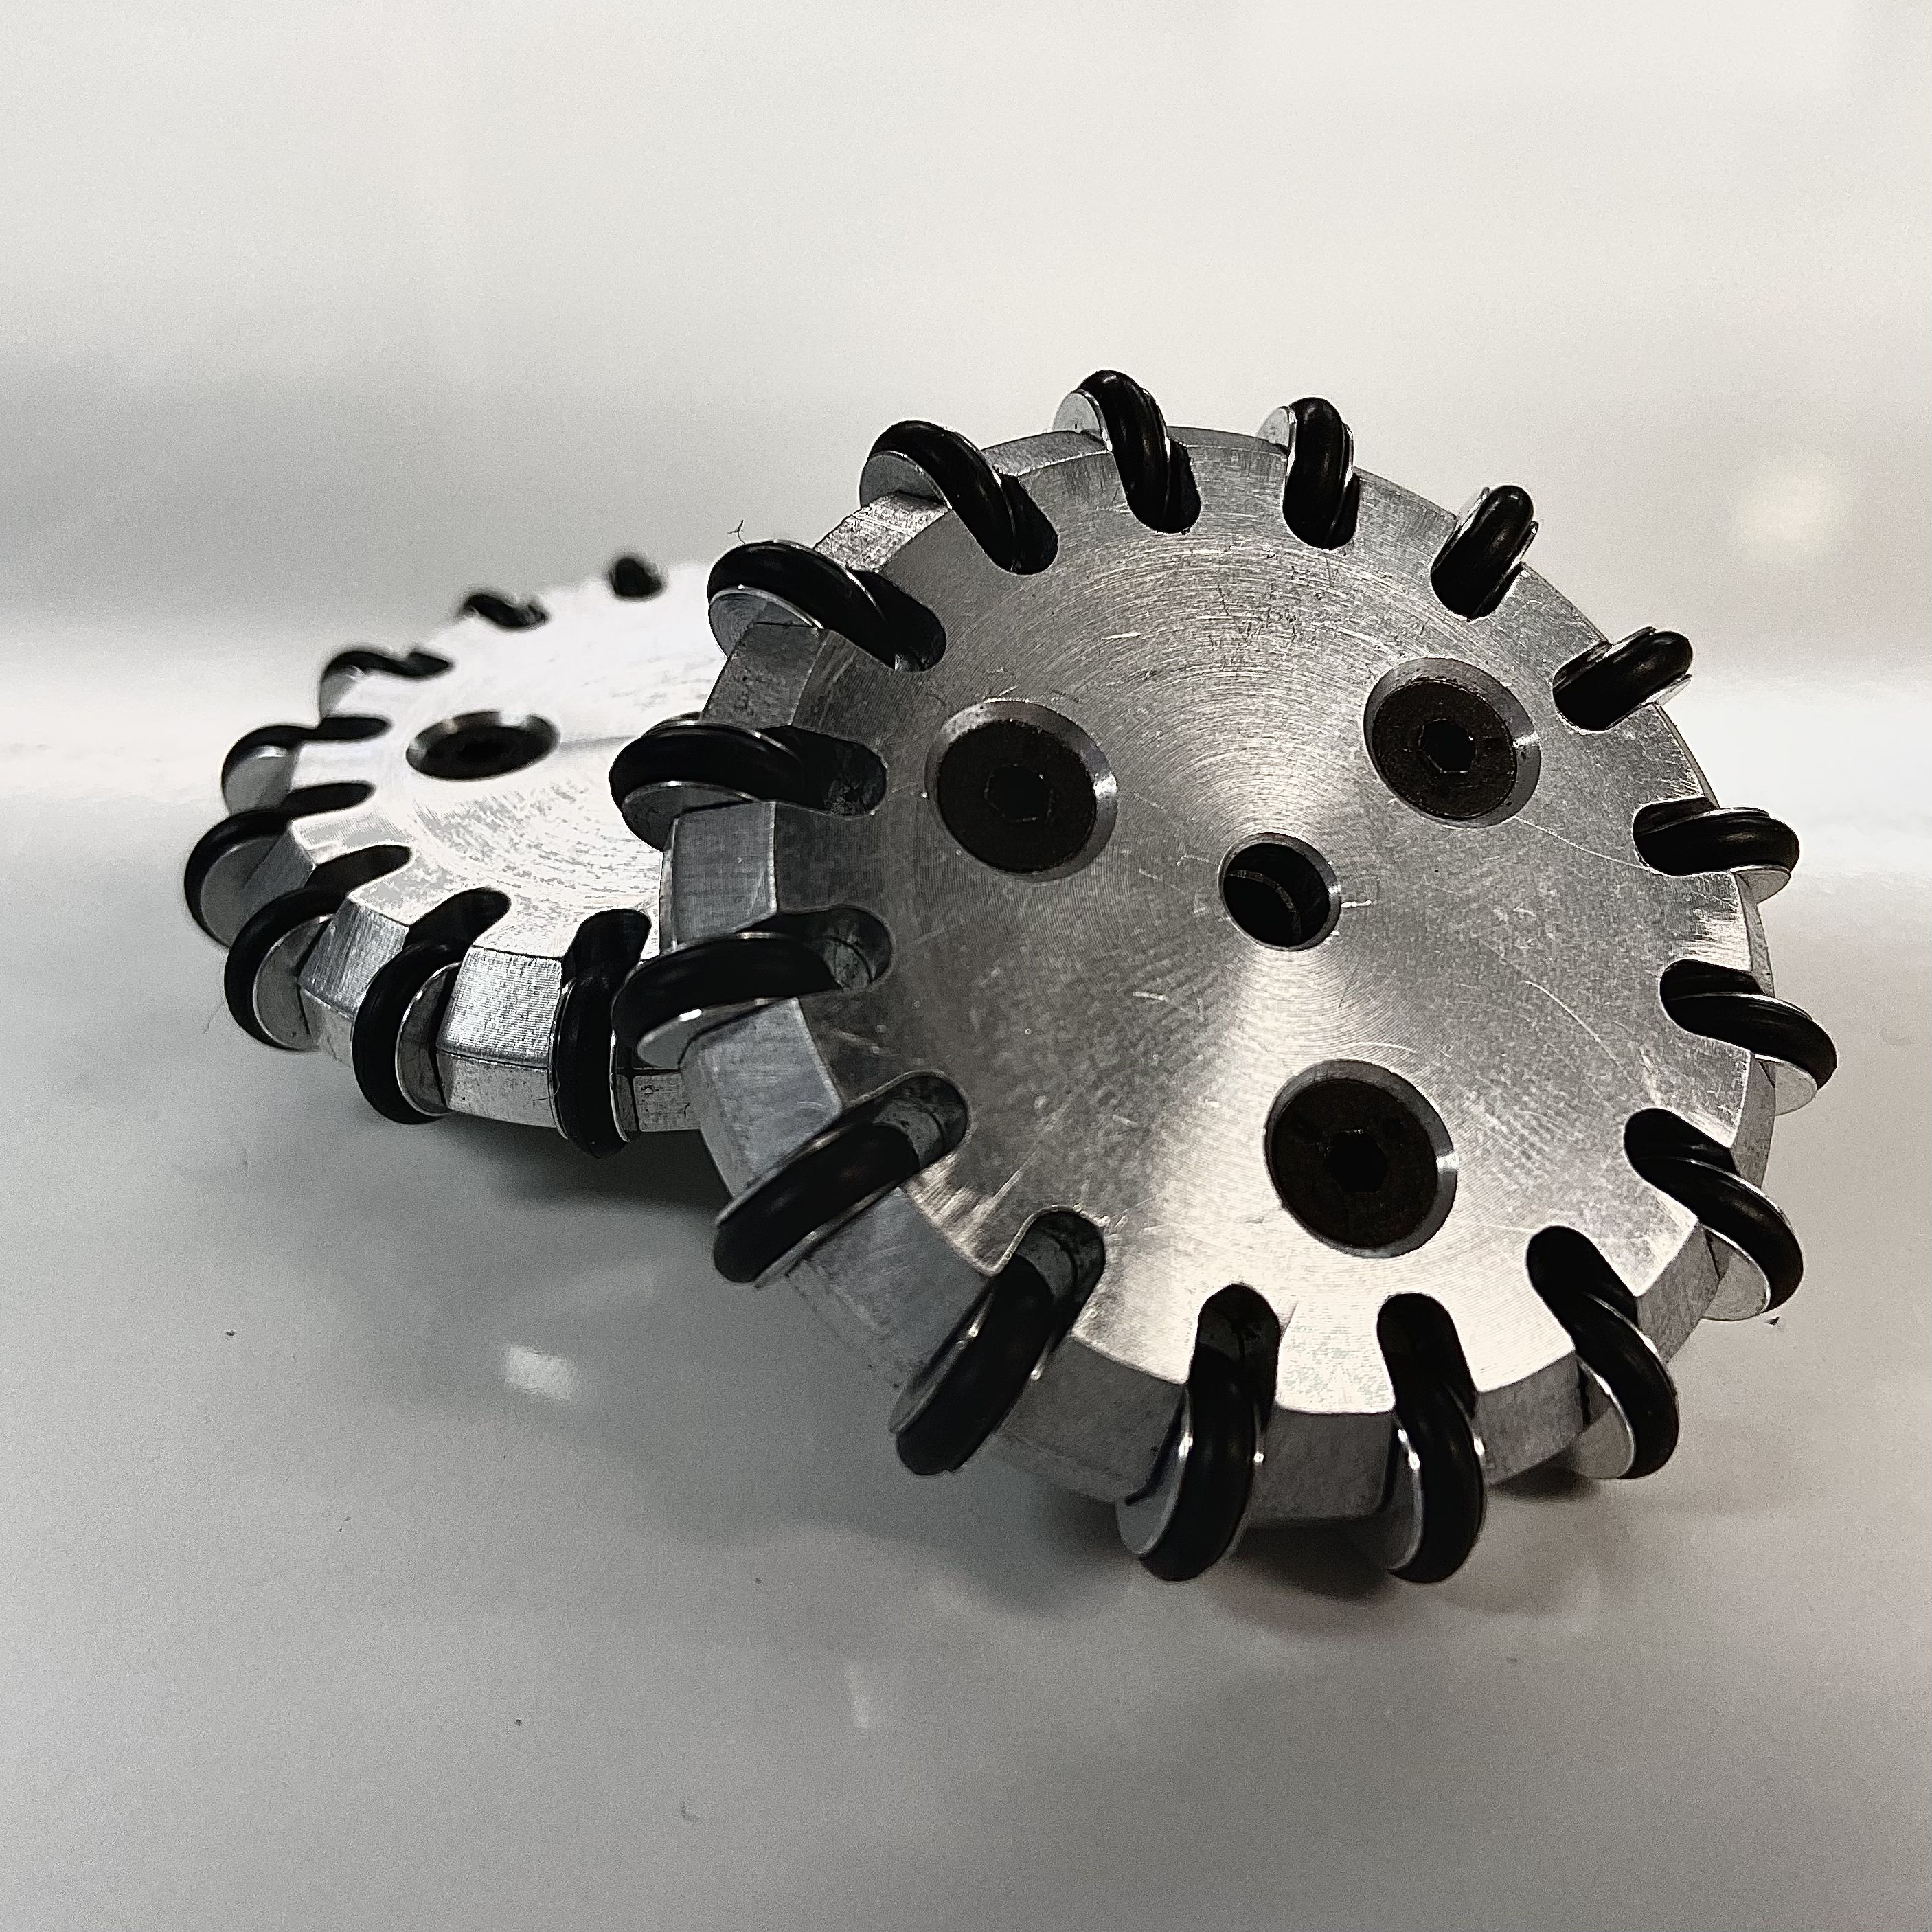
\includegraphics[width=1\linewidth]{img/inv/OmniWheel.jpg}
    \caption{Omniwheels}
    \label{fig:OmniWheels}
\end{wrapfigure}

The whole design aims to be fast, reliable and robust. To achieve this goal, we put all the force
into two Carbon Rings. Carbon Fiber has a high strength and low weight.
\newline
Traveling with high speeds, while being strong is also a huge challenge. To achieve this, we use high quality
Maxon DC Motors in combination with the VNH3SP30 driver chip. To put the force on the ground, we designed
new Omniwheels.
The OmniWheel consists of two independent aluminum pieces screwed together. For the small wheels we use a small
aluminum piece covered with an O-Ring out of EPDM plastic.
\newline
To protect this whole construction from the opponent robot, everything is moved 1.5 cm into the robot and a 3D
printed protector covers the whole inner side of the robot.
\newline

\subsection{Electrical Design}
To detect various elements and control the whole robot we use a Teensy 4.1 microcontroller. All electronic
parts are soldered to circuit boards.
\newline
We have a total of four Circuit Boards:
\begin{enumerate}
    \item{Line Detection PCB} \label{PCB:LD}
    \item{Step Up PCB} \label{PCB:SU}
    \item{Controller PCB} \label{PCB:C}
    \item{Infrared Seeker PCB} \label{PCB:IS}
\end{enumerate}
Each Circuit Board has a predetermined task and all the above are controlled by the Teensy 4.1.

We order our Circuit Boards from a local company and solder the parts on the boards.

\subsubsection{Line Detection PCB}

\begin{wrapfigure}{r}{4cm}
    \centering
    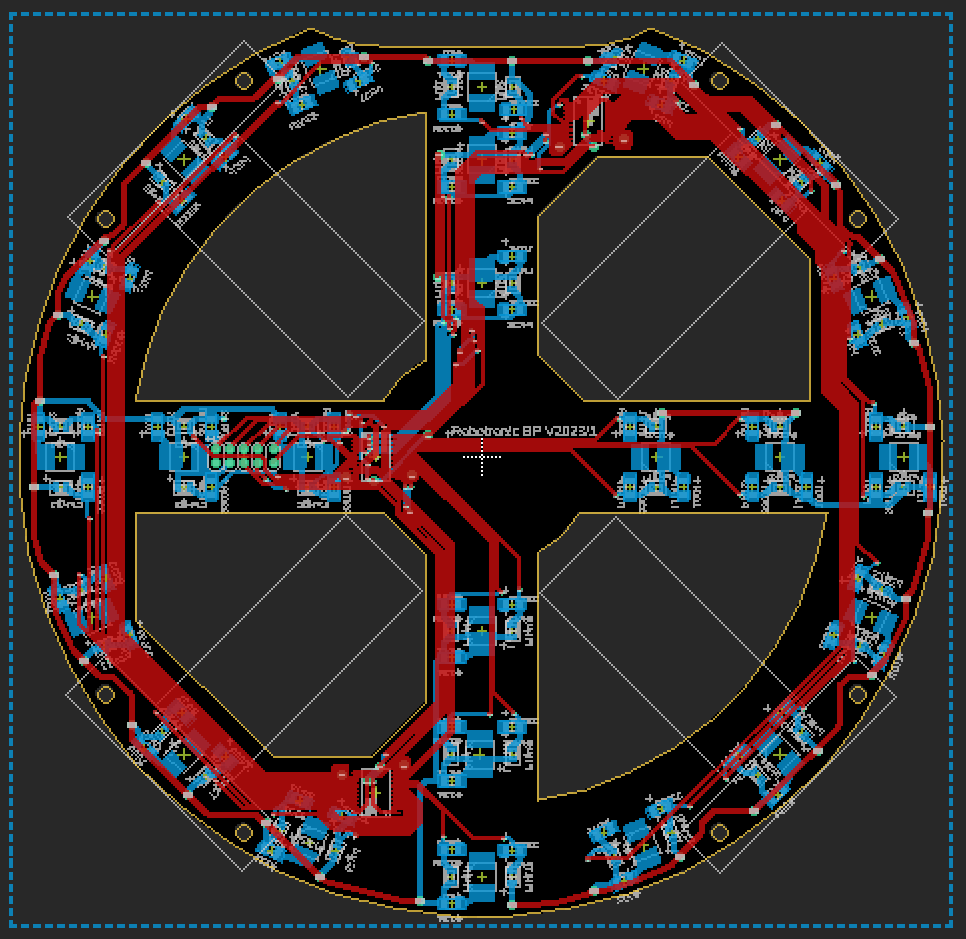
\includegraphics[width=0.75\linewidth]{img/eagle/LineDedectionPCB.png}
    \caption{PCB}
    \label{fig:LDPCB}
\end{wrapfigure}

\ref{PCB:LD} The Line Detection PCB consists of a circle and a cross of phototransistor pairs. To connect all
48 sensors to our main controller, we use analog multiplexer. The multiplexers are switched parallel
to save ports.
\newline
As you can see on the right, we use pairs of two phototransistors and one led. We found out, this is the 
best way to detect the line.

\subsubsection{Step Up PCB}
\ref{PCB:SU} Because a simple solenoid with 12V isn't strong enough, we use a selfmade 
StepUp converter. It consists of a controller and a coil to convert the 12V
to 48V - the maximum allowed.
\newline

\subsubsection{Controller PCB}

\begin{wrapfigure}{r}{5cm}
    \centering
    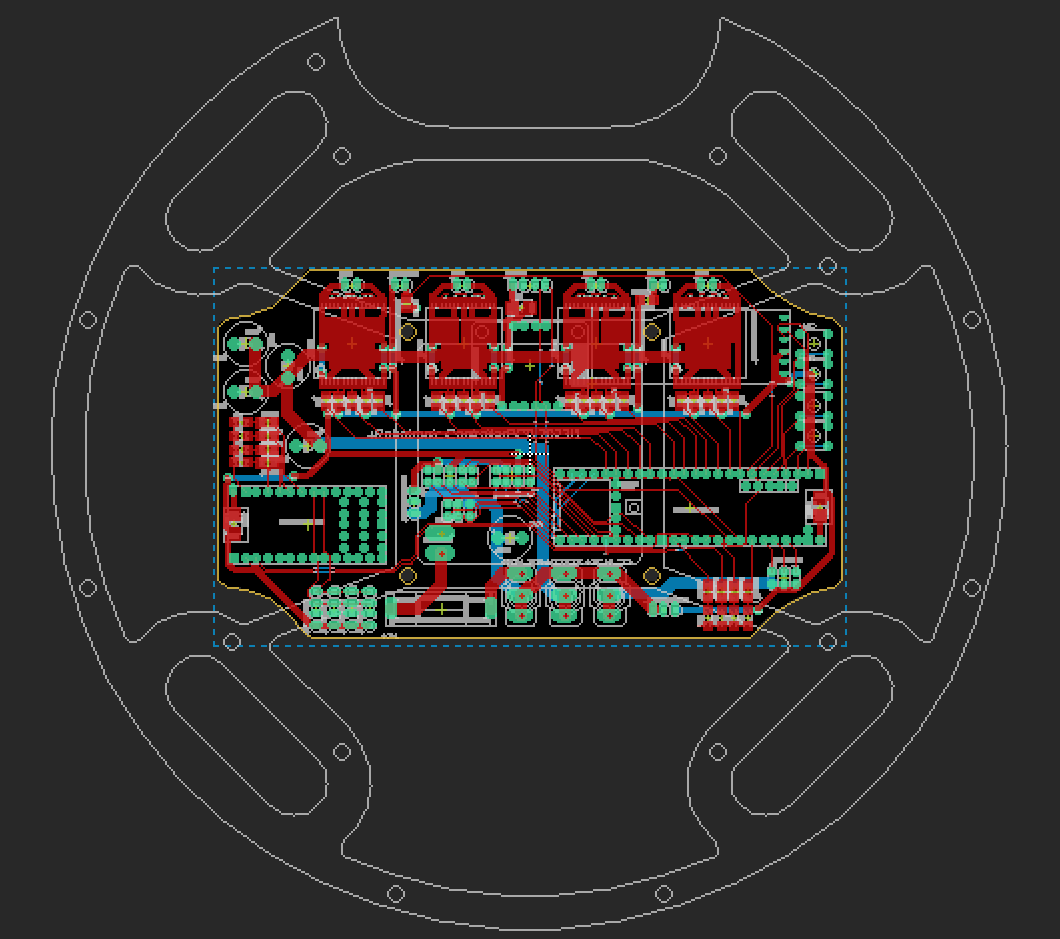
\includegraphics[width=0.75\linewidth]{img/eagle/ControllerPCB.png}
    \caption{PCB}
    \label{fig:CPCB}
\end{wrapfigure}

\ref{PCB:C} To control our whole robot we have a circuit board with two microcontrollers. One Teensy 4.0 and one Teensy 4.1. The 4.0 is to communicate with
mouse sensor over SPI. The Teensy 4.1 controls our motors, reads the values from all multiplexers and the compass sensor. The communication is also 
handled by the Teensy 4.1. 
\newline
As you can see on the right~\ref{fig:CPCB}, the power management is also done on the controller PCB.
\newline

For on the way debug, we have a total of eight small SMD-LED´s on our circuit board.
Each is light up, if an specific condition is reached.
\begin{enumerate}
    \item{Cameras are functioning correctly}
    \item{Compass direction equals robot direction}
    \item{IR Ball is detected}
    \item{Line is detected}
\end{enumerate}

\hfill \break
For changes on the flight, we also have four buttons. 
\begin{enumerate}
    \item{Calibration of robot}
    \item{Shoot test}
    \item{Delete previous IR-Calibration and start scanning for new one}
    \item{Save new IR values}
\end{enumerate}
\hfill \break

We put as much as possible on this circuit board, to save space and weight.

\subsubsection{Infrared Seeker PCB}

\begin{wrapfigure}{l}{5cm}
    \centering
    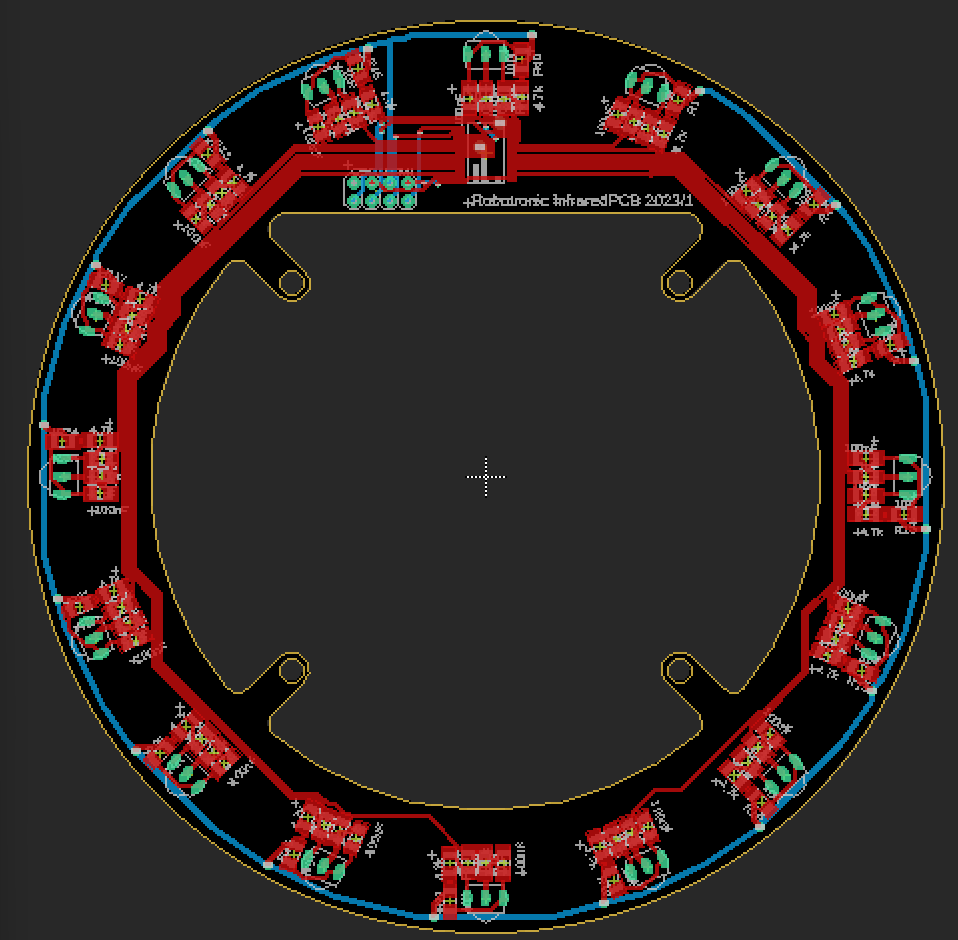
\includegraphics[width=0.75\linewidth]{img/eagle/IrSeekerPCB.png}
    \caption{PCB}
    \label{fig:ISPCB}
\end{wrapfigure}

\ref{PCB:IS} To detect the ball as fast, reliable and precise as possible
our IR Seeker circuit board consists out of a ring with a total of 16 TSSP4038,
all connected with a multiplexer chip. 
\newline
The TSSP4038 are the most commonly used IR sensors in the RoboCup Junior LightWeight
league. But instead of using the direct output, we convert it to an analog signal
With this method, we can detect an approximate distance to the ball. Our total speed
depends on this distance, as closer we get, the slower we drive, to enhance the accuracy. 
\newline 

\subsection{Software} %hier muss noch UNDBEDINGT, zwischen Torwart und Stürmer unterschieden werden.
As we all know, that's the objective:
\begin{enumerate}
    \item{Approach the ball quickly and precisely to get it into the ball pit.}
    \item{Aim for the goal as quickly as possible.}
    \item{Score as fast as possible.}
\end{enumerate}
Accordingly, a modularization of the code can be set up.

\subsubsection{Ball approach}
Our idea was to set up an imaginary approach circle around the ball, which is then approached tangentially. The speed is to be controlled in the process.
On the one hand, with the distance tot the ball and the targeted distance of the radius of the imaginary circle.
On the other hand, with the angle, whereby the aim is to place the robot exactly behind the ball. 
The output of the PID controllers wa s transferred to the motor formula with a convex combination via the distance to the ball.

If the ball is now in front of the robot, it is driven straight ahead until the ball is registered in the ball pit with the light barrier. Then the next module is activated.

\subsubsection{Aiming at the goal}
As long as the ball is in the ball pit, the robot aligns itself with the goal and drives up to a suitable shooting position. To prevent \textit{pushing}, the shot is taken as early as possible.

\subsubsection{Shot}
The standard shot consists of the bolt, which accelerates the ball and is subject to the rules. In conjunction with an aggressive spin, the ball can be catapulted forward much more.

\subsection{Steering with mouse sensor}
To be able to achieve the above, it is of course inherent to be able to control effectively, robustly and precisely.
The necessary target/actual comparison is done with the help of a mouse sensor.
This registers the current speed and the current direction of movement (this is similar to polar coordinates). A PID controller now controls the motors.

\subsection{Ball detection and infrared light}
For each individual infrared sensor, the pulsing of the ball is integrated over a short period of time and thus the distance is estimated.
To compensate for hardware differences, the sensors are calibrated to the ball before each game. This calibration is stored and automatically improves over the course of a game. 

The sensor with the shortest distance to the ball then represents the angle to the ball. This is therefore dependent on the placement of the sensors on the robot.

\subsection{Goal detection and camera}
The distance to the goal is determined by the height of the largest blue/yellow block.
The angle to the goal, which is aligned with the ball approach and the passive goalkeeper, is the angle to the center of the largest block. 

\subsection{Line detection}
Automatic calibration of the ground sensors at the beginning of each game lets us react quickly to all lighting conditions. 
If a phototransistor detects a larger light value than the initially calibrated value, a countersteering vector is passed to the motor formula. 
This vector depends on the hardware position. This remains even if another sensor detects a line in the near future.

\subsection{Goalkeeper}
Our storm is more effective when it consists of only one robot. The other one should cover as much area of the goal as possible.
This goalkeeper moves on his own penalty line and navigates between the ball and the center of the goal, so that either \textit{pushing} is triggered, or a shot is blocked.
The goalkeeper's offense can be adjusted, as he can decide when to drive on the ball. 

\subsection{Bluetooth}
An effective goalkeeper change completes our tactics. This is ensured with an economical Bluetooth protocol, so that one robot is always the goalkeeper and the other the striker. 